\documentclass[12pt,parskip=half-, twoside=semi]{scrartcl}
\usepackage[T1]{fontenc} % encodage des caractères
\usepackage[french]{babel} % texte en français
\usepackage{microtype} % meilleur justification du texte
\usepackage{cmbright} % police sans serif
\usepackage[frenchmath]{mathastext} % pour le lettres majuscules droites
\usepackage{stmaryrd} % \sslash pour le symbole parallèle
\usepackage{mathtools}
\usepackage{graphicx}
\usepackage{tikz, tkz-euclide}
\usepackage{enumitem}
\setlist[enumerate]{label=\alph*)}
\usepackage{tcolorbox}
\usepackage{gensymb}
\usepackage{tabularray}
\newcolumntype{Y}{>{\centering\arraybackslash}X}
\usepackage{tabularx}
\usepackage{multicol}
\SetEnumitemKey{cols}
{
    itemsep= 1em,
    before = \raggedcolumns\begin{multicols}{#1},
    after = \end{multicols},
}
\usepackage{tcolorbox}
\newtcbox{\blackbox}{%
    on line,
    left=0pt,
    right=0pt,
    bottom=0pt,
    top=0pt,
    sharp corners,
    colframe=black,
    colback=black,
    coltext=white,
    fontupper=\bfseries
}
\usepackage[use-files, use-aux]{xsim}
\DeclareExerciseEnvironmentTemplate{interrogation_template}%
{%
    \GetExercisePropertyTF{points}%
    % s'il y a des points
    {
        \blackbox%
        {%
            \XSIMmixedcase{\GetExerciseName}~\GetExerciseProperty{counter}%
        }%
        \hfill
        \blackbox{
            \GetExerciseProperty{points}
        }
        \par
    }
    % sinon
    {
        \blackbox%
        {%
            \XSIMmixedcase{\GetExerciseName}~\GetExerciseProperty{counter}%
        }%
        \par
    }%
}%
{%
    \par%
}
\xsimsetup{
    exercise/template = interrogation_template,
    solution/template = interrogation_template,
    exercise/name = question,
}

\begin{document}
Nom et prénom : \\
Classe : \\

\begin{huge}
    \begin{center}
        Révisions de mathématiques - 1ère année \\
    \end{center}
\end{huge}
    
\begin{center}
    \textit{Á réaliser sur une feuille annexe, à l'exception des exercices présicés dans l'énoncé.}
\end{center}

\begin{exercise}
    Donne la nature des quadrilatères ci-dessous. \\
    \begin{center}
      
\includegraphics[width=4cm]{quadri.png}    
    \end{center}
\end{exercise}

\begin{exercise}
    Effectue.
    \begin{enumerate}[itemsep=1cm, cols=5]
        \item $1^3$
        \item $5^2$
        \item $\left(-2\right)^3$
        \item $\left(-3\right)^2$
        \item $-1^6$
        \item $\left(-1\right)^6$
        \item $2^4$
        \item $-2^4$
        \item $\left(-2\right)^4$
        \item $\left(-5\right)^3$
        \item $3^1$
        \item $5^0$
        \item $-3^3$
        \item $\left(-6\right)^2$
        \item $0^2$
    \end{enumerate}
\end{exercise}

\begin{exercise}
    Range les nombres suivants dans l'ordre croissant. 
    \begin{enumerate}[cols = 7, label=]
        \item -2,3
        \item 4
        \item -3,2
        \item 4,1
        \item -3,5
        \item 4,6
        \item 0
    \end{enumerate}
\end{exercise}

\newpage
\begin{exercise}
    Donne le nom de la propriété utilisée dans chacune des égalités suivantes. 
    \begin{enumerate}[cols=2]
        \item $5 \cdot 0 = 0$ 
        \item $59 + 2= 2 + 59$ 
        \item $4 \cdot 2 \cdot 3 = 3\cdot 2 \cdot 4$ 
        \item $5 + 2 + 6 = 5 + \left(2+6\right)$ 
    \end{enumerate}
\end{exercise}

\begin{exercise}
    \textbf{Sur cette feuille.} Indique d'une croix dans la/les case(s) adéquate(s).\\
    {\renewcommand{\arraystretch}{1.4}
    \begin{tabularx}{\linewidth}{|p{1.5cm}|Y|Y|Y|Y|}
        \hline
        & est divisible par & est un diviseur de & divise & est un multiple de \\
        \hline
        $6 \dots 24$ & & & &\\
        \hline
        $24 \dots 8$ & & & &\\
        \hline
        $20 \dots 20$ & & & & \\
        \hline
        $0 \dots 15$ & & & & \\
        \hline
    \end{tabularx}}
\end{exercise}

\begin{exercise}
    Cite les nombres naturels qui sont \dots
    \begin{enumerate}[cols=2]
        \item diviseurs de 30
        \item multiples impairs de 7 inférieurs à 50
        \item multiples pairs de 3 inférieurs à 25
        \item diviseurs de 100 multiples de 5
    \end{enumerate}
\end{exercise}

\begin{exercise}
    Construis un triangle en sachant qu'un de ses angles mesure $80\degree$ et que les côtés adjacents à cet angle mesurent 4 cm et 6 cm.
\end{exercise}

\begin{exercise}
    Voici un programme de calcul dont le résultat est -4. Retrouve le nombre de départ, et laisse ta démarche visible.

    \begin{center}
        \begin{minipage}{6cm}
        \begin{tcolorbox}
            Choisis un nombre. \\ Ajoute-lui 7. \\ Multiplie le résultat par 2. \\ Enlève 6 au résultat. 
         \end{tcolorbox}
     \end{minipage} 
    \end{center}
\end{exercise}

\begin{exercise}
    Complète les phrases suivantes par les mots proposés : hauteur, médiane, médiatrice, bissectrice, diagonale.
        \begin{center}
           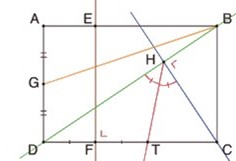
\includegraphics[width=5cm]{img/droitesrema.jpg} 
        \end{center}
    \begin{enumerate}
        \item La droite $BD$ est une \ldots du rectangle $ABCD$.
        \item La droite $CH$ est une \ldots du triangle $BCH$.
        \item La demi-droite $ [HT $ est une \ldots du triangle $CHD$.
        \item Le segment de droite $[GB]$ est une \ldots du triangle $ABD$.
        \item La droite $EF$ est une \ldots du triangle $DTH$.
    \end{enumerate}
\end{exercise}

\begin{exercise}
    Les figures ci-dessous ont été dessinées à main levée. Reproduis-les en respectant les mesures indiquées. 
    \begin{center}
        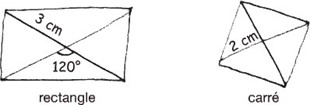
\includegraphics[]{img/quadri.jpg}
    \end{center}
\end{exercise}

\begin{exercise}
    Construis un triangle en sachant qu'un de ses côtés mesure 7 cm et que les angles adjacents à ce côté mesurent $45\degree$ et $60\degree$.
\end{exercise}

\begin{exercise}
    Calcule.
    \begin{enumerate}[cols=2]
        \item $2^2+5^2$
        \item $3^3-3^2$
        \item $2^2+5^3$
        \item $-2\cdot 4^2$
        \item $2 + \left(5+\left(-2\right)\right) \cdot 3$
        \item $5^2 - 30$
    \end{enumerate}
\end{exercise}

\begin{exercise}
    Pour les cadeaux de Noël, Amélie a acheté 5 CD à la Fnac. Au moment de payer, elle a sorti un billet de 100€ de son portefeuille, mais le caissier lui a fait gentiment remarquer qu’il manque 12€. Calcule le prix de vente d’un CD en laissant ta démarche visible.
\end{exercise}

\begin{exercise}
    Le triangle ci-dessous a été dessiné à main levée. Reproduis-le en respectant les mesures, puis trace toutes ses hauteurs en vert. \\ Code ton dessin.
    \begin{center}
        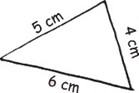
\includegraphics[]{img/tri.jpg}
    \end{center}
\end{exercise}

\begin{exercise}
    Le triangle ci-dessous a été dessiné à main levée. Reproduis-le en respectant les mesures, puis trace toutes ses médianes en bleu. \\ Code ton dessin.
    \begin{center}
        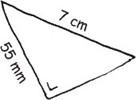
\includegraphics[]{img/tri2.jpg}
    \end{center}
\end{exercise}

\begin{exercise}
    \textbf{Sur cette feuille.} Parmi les solides suivants, 
    \begin{enumerate}
        \item Barre ceux qui ne sont pas des prismes droits.
        \item Pour ceux qui restent, colorie une base en vert, une hauteur en bleu et une face latérale en rouge.
        \item [\label=] 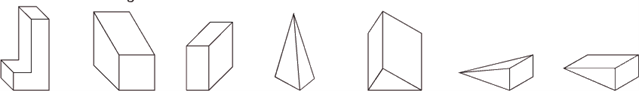
\includegraphics[]{img/prismes.png}
    \end{enumerate}
\end{exercise}

\begin{exercise}
    Construis un losange $ABCD$ en sachant que $|\widehat{A}|=60\degree$ et que son périmètre vaut 16 cm.
\end{exercise}

\begin{exercise}
    Décode. 
    \begin{enumerate}[cols=3]
        \item $5+\left(-2\right)$
        \item $8^3+3$ 
        \item $t_{\overrightarrow{v}} ([AC])= [A'C']$
    \end{enumerate}
\end{exercise}

\begin{exercise}
    \textbf{Sur cette feuille}. Trace l'image des points $A, B$ et $C$ par la symétrie orthogonale d'axe $d$. Laisse tes constructions visibles.
    \begin{center}
        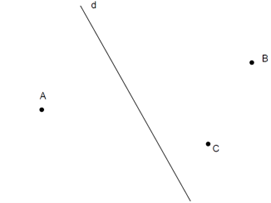
\includegraphics[]{img/symportho.png}
    \end{center}
\end{exercise}

\begin{exercise}
    Construis un parallélogramme $ABCD$ si tu sais que $|AC|=6 cm$, $|BD|=4 cm$, $M$ est l'intersection des diagonales et $|\widehat{DMA}| = 70\degree$.
\end{exercise}

\begin{exercise}
    Calcule les valeurs numériques des expressions suivantes.
    \begin{enumerate}[itemsep=1cm, cols=2]
        \item $23+t-4t$ si $t=4$
        \item $3c^2-c+10$ si $c=-2$
        \item $3\left(60 -p\right)$ si $p=40$
        \item $a + 2b -10ab$ si $a=2$ et $b=-3$
    \end{enumerate}
\end{exercise}

\begin{exercise}
    \textbf{Sur cette feuille.} Le solide suivant est un prisme droit à base hexagonale. \\
    Complète par le symbole adéquat (utilise "G" pour "gauche").
    \begin{enumerate}[cols=3]
        \item [\label=] 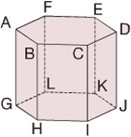
\includegraphics[]{img/prismehexa.jpg}
        \item $[HI] \ldots [IJ]$
        \item $[CI] \ldots [AG]$
        \item $[HI] \ldots [AG]$
        \item $[BC] \ldots [LK]$
        \item $AFLG \ldots CDJI$
        \item $ABHG \ldots EDJK$
        \item $LKJIHG \ldots LKEF$
        \item $AFLG \ldots EDJK$
    \end{enumerate}
\end{exercise}

\begin{exercise}
    Justifie chaque proposition ci-dessous en utilisant un caractère de divisibilité.
    \begin{enumerate}[cols=2]
        \item 126 est divisible par 3
        \item 492 est divisible par 4
        \item 135 est divisible par 5
        \item 2432 est divisible par 8 
    \end{enumerate}
\end{exercise}

\begin{exercise}
    Voici le croquis d'une armoire d'angle (entre deux murs, donc en faisant un angle de $90\degree$) fabriquée par mon grand-père. Calcule le volume de cette armoire. 
    \begin{center}
        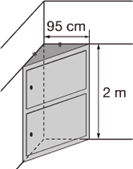
\includegraphics[]{img/armoire.png}
    \end{center}
\end{exercise}

\begin{exercise}
    Donne l'ensemble des 10 premiers multiples de 12.
\end{exercise}

\begin{exercise}
    Donne l'ensemble des diviseurs de 24.
\end{exercise}

\newpage
\begin{exercise}
    \textbf{Sur cette feuille.} Dans le repère suivant \dots \\
    \begin{enumerate}
        \item [\label=] 
\includegraphics[]{img/repere.png}
        \item Détermine les coordonnées des points suivants.
        \begin{enumerate}[cols=3, label=]
            \item $A$
            \item $B$
            \item $C$
            \item $D$
            \item $E$
            \item $F$
            \item $G$
            \item $H$
        \end{enumerate}
        \item Place les points dont voici les coordonnées.
        \begin{enumerate}[cols=6, label=]
            \item $X\left(2;5\right)$
            \item $Y\left(-3;2\right)$
            \item $Z\left(4:-3\right)$
            \item $W\left(-2;-1\right)$
            \item $T\left(4;0\right)$
            \item $U\left(0;-3\right)$
        \end{enumerate}
    \end{enumerate}
\end{exercise}

\begin{exercise}
    Que vaut $m$ dans les équations suivantes? Utilise les chaines d'opérations et laisse ta démarche visible.
    \begin{enumerate}[cols=2]
        \item $4m+2=82$
        \item $3\left(m-2\right)=15$
        \item $21=3m+6$
        \item $\left(3+2m\right)\cdot 2=22$
    \end{enumerate}
\end{exercise}

\newpage
\begin{exercise}
    Observe la suite suivante. 
    \begin{center}
        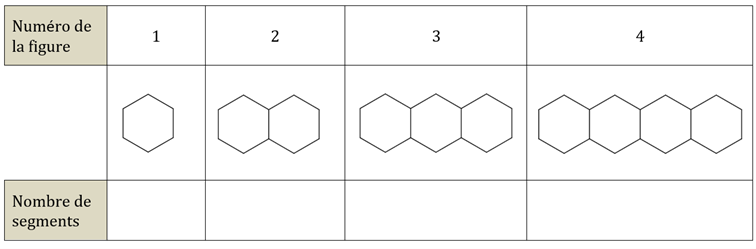
\includegraphics[]{img/suite.png}
    \end{center}
    \begin{enumerate}
        \item \textbf{Sur cette feuille.} Complète le tableau suivant. \\
        {\renewcommand{\arraystretch}{2}
        \begin{tabularx}{\linewidth}{|p{4cm}|Y|Y|Y|Y|Y|Y|Y|}
            \hline
            Numéro de la figure & 1& 2& 3& 4& 5& 6& $n$\\
            \hline
            Nombre de cubes & & & & & & & \\
            \hline
        \end{tabularx}}

        \item Combien de cubes composeront\dots
        \begin{enumerate}
            \item \dots la 10ème figure?
            \item \dots la 312ème figure?
        \end{enumerate}
        \item Quel est le numéro de la figure qui est composée de 972 cubes? Laisse ta démarche visible.
    \end{enumerate}
\end{exercise}

\begin{exercise}
    Calcule, sans t'aider de la calculatrice.
    \begin{enumerate}[cols=2]
        \item $50\%$ de $48$
        \item $5\%$ de $80$
        \item $75\%$ de $12$
        \item $10\%$ de $60$
    \end{enumerate}
\end{exercise}

\begin{exercise}
    Calcule, en utilisant éventuellement la calculatrice.
    \begin{enumerate}[cols=2]
        \item $12\%$ de 14 500.
        \item 21\% de 45 000.
        \item 25\% de 145.
        \item 7,5\% de 650.
    \end{enumerate}
\end{exercise}

\begin{exercise}
    \textbf{Sur cette feuille.} Encadre en utilisant des nombres entiers consécutifs.
    \begin{enumerate}[cols=2, label=]
        \item $\ldots < 5,4 < \dots$
        \item $\ldots < 0,5 < \dots$
        \item $\ldots < -4,8 < \dots$
        \item $\ldots < -1,5 < \dots$
    \end{enumerate}
  \end{exercise}
  
  \begin{exercise}
      Calcule.
      \begin{enumerate}[cols=3]
          \item $-5 + (-6) $
          \item $5 \cdot (-9) $
          \item $5 - 9 $
          \item $(-2)^3 $
          \item $-13 + 64 - (-3)^3 $
          \item $12 - 20 $
          \item $-2\cdot (-3) $
          \item $-6 + 2 + 9 - 8$
          \item $-5\cdot (-6) \cdot 9 \cdot 2 $
          \item $12 - 15 - 13 $
          \item $38 + 14 - 24 + 6 $
          \item $12\cdot (-8) \cdot 5\cdot (-2) $
          \item $-34 + 84 - 15 + 18 $
          \item $100 \cdot (-4) \cdot 2 \cdot (-5) $
          \item $-100 - 4 + 2 - 5 $
      \end{enumerate}
  \end{exercise}

\begin{exercise}
    Voici la répartition des dépenses mensuelles d'un ménage. Représente cette répartition à l'aide d'un diagramme circulaire, et n'oublie pas la légende ! 
    \begin{enumerate}[cols=3, label=]
        \item Logement : 688€
        \item Loisirs : 245€
        \item Alimentation : 539€
        \item Transports : 343€
        \item Habillement : 441€
        \item Santé : 196€
    \end{enumerate}
\end{exercise}

\begin{exercise}
    Une enquête a été réalisée au sein d'une école pour connaitre le temps hebdomadaire moyen consacré au sport. Voici (en minutes) les résultats obtenus par année. Représente cette situation à l'aide d'un diagramme en bâtonnets.
    \begin{enumerate} [cols=3, label=]
        \item 1ère année : 160
        \item 2ème année : 120
        \item 3ème année : 310
        \item 4ème année : 150
        \item 5ème année : 330
        \item 6ème année : 70
    \end{enumerate}
\end{exercise}

\begin{exercise}
    Invente des coordonnées pour le point $P$ si tu sais que son ordonnée est égale à l'opposé de son abscisse, augmenté de 1.
\end{exercise}

\begin{exercise}
    Décompose les nombres suivants en un produit de facteurs premiers. 
    \begin{enumerate}[cols=4]
        \item 36
        \item 196
        \item 432
        \item 100
    \end{enumerate}
\end{exercise}

\begin{exercise}
    Lorsqu’il va chez son oculiste, Monsieur Leborgne paie 75€ pour la consultation. Sa mutuelle lui rembourse 70\% de ce montant. Sur le montant restant à sa charge après remboursement de la mutuelle, son assurance « soins de santé » lui rembourse 80\%. \\
Quel pourcentage du prix de la consultation a-t-il finalement payé ? Laisse ta démarche visible.
\end{exercise}

\begin{exercise}
    Pour le cocktail d’anniversaire de Maria, il est noté ce qui suit : 

Pour 10 personnes :
\begin{enumerate}[label=-]
    \item 120 cl d’eau pétillante 
    \item 50g de sucre glace
    \item 20 cl de grenadine
    \item 1 demi citron
    \item 160cl de sprite
\end{enumerate}
Maria compte faire ce cocktail pour les 12 personnes présentes à la fête. Calcule les quantités nécessaires de chacun des aliments. Laisse ta démarche visible.
\end{exercise}

\begin{exercise}
    Range les nombres suivants dans l'ordre croissant. 
    \begin{enumerate}[cols = 7, label=]
        \item -7
        \item 6
        \item -4
        \item -6
        \item 5
        \item 10
        \item -15
    \end{enumerate}
\end{exercise}

\newpage
\begin{exercise}
    \textbf{Sur cette feuille.} Complète les couples de coordonnées suivantes pour que l'abscisse soit toujours le consécutif de l'ordonnée. 
    \begin{enumerate}[cols=4, label=]
        \item $A\left(5; \ldots\right)$
        \item $M\left(-2; \ldots \right)$
        \item $I\left(\ldots ; -8\right)$
        \item $S\left(\ldots ; 0\right)$
    \end{enumerate}
\end{exercise}

\begin{exercise}
    Calcule en utilisant les règles de priorité des opérations.
    \begin{enumerate}[cols=3]
        \item $	5 - 2 \cdot 8$
        \item $-5 - 2 \cdot 8 - 9$
        \item $-7 \cdot(-2)+ 5 \cdot 3$
        \item $-3^2 + 5 \cdot (-2)$
        \item $(5 - 9 )\cdot(3 - 7)$
        \item $5 - 9 \cdot(3 - 7)$
        \item $ 1 + 4^2- 2 \cdot (-3)^2$
        \item $ 1+ 4 \cdot ( -2 + 2^2 )$
        \item $(2 - 5 )^3 \cdot (2 - 8 )^2$
    \end{enumerate}
\end{exercise}

\begin{exercise}
    Calcule les valeurs numériques des expressions suivantes si tu sais que \\ $a=-2, b=3, c=-5$ et $d=4$
    \begin{enumerate}[cols=3]
        \item $	a + b$
        \item $7c $
        \item $-3d $
        \item $3a + 2b$
        \item $-2c - 3d $ 
        \item $6(c + d)$ 
        \item $-3(c - a )$ 
        \item $a^2$
        \item $3b^3$
        \item $3a^2-2\cdot \left(c+d\right)$
    \end{enumerate}
\end{exercise}

\begin{exercise}
    \textbf{Sur cette feuille.} Le tableau ci-dessous donne les températures extrêmes observées pendant une année dans différentes villes du monde. Pour chacune, calcule l'écart entre les deux températures extrêmes. \\
    {\renewcommand{\arraystretch}{1.4}
    \begin{tabularx}{\linewidth}{|Y|Y|Y|Y|}
        \hline
        Ville & Maximum (\degree $C$) & Minimum (\degree $C$) & Écart \\
        \hline
        \hline
        Corinthe & 42 & 2 & \\
        \hline
        Budapest & 25 & -9 & \\
        \hline
        Dakar & 46 & 8 & \\
        \hline
        Bruxelles & 29 & -8 & \\
        \hline
        Montréal & 21 & -13 & \\
        \hline
    \end{tabularx}}
\end{exercise}

\begin{exercise}
    Si possible, réduis au maximum les expressions suivantes.
    \begin{enumerate}[cols=3]
        \item $-b-b$
        \item $4a\cdot \left(-b\right)$
        \item $-2a^2 - 5a$
        \item $-2a\cdot \left(-5a\right)$
        \item $b^2-5b$
        \item $2b-6b+4a$
        \item $b^2 - 5b^2$
        \item $a\cdot \left(-2b\right) \cdot \left(-3c\right)$
        \item $-2b + 5b$
        \item $2a\cdot \left(-5b\right)$
        \item $am \cdot am \cdot a^3 \cdot m^2$
        \item $3a\cdot \left(-5a\right) \cdot \left(-6b\right)$
    \end{enumerate}
\end{exercise}

\begin{exercise}
    Enlève les parenthèses et réduis au maximum.
    \begin{enumerate}[cols=2]
        \item $-a + (-b - c) $
        \item $3\cdot (2x + 2 )$
        \item $- (3x - 2y) +(x - y) $
        \item $(x + 4y) \cdot 2x $
        \item $-2 + (a + 4) - (-3 + a)$
        \item $2a\cdot (2a-5b)+12ab $
        \item $x^2-(5x^2 -2x + 3) $ 
        \item $(5a +5)- (4 + 3a) $ 
        \item $3+(x-5)+(x^2-5x) $ 
        \item $5a+(5-a)\cdot 4 $
    \end{enumerate}
\end{exercise}

\begin{exercise}
    Factorise en utilisant la mise en évidence.
    \begin{enumerate}[cols=3]
        \item $2x + 2y$
        \item $5ac - 5ad $
        \item $3+ 3a $
        \item $2a - 8b $
        \item $5b + 25c$
        \item $12 ab+ 15 bc$
        \item $4 abx - 6 aby $
        \item $20 ab + 10a$
        \item $4a^3 - 5a^2b$
    \end{enumerate}
\end{exercise}

\begin{exercise}
    Trace un cercle de centre $O$ et de rayon de 4 cm. Construis un hexagone régulier inscrit dans ce cercle. \\ Laisse ta démarche visible.
\end{exercise}

\newpage
\begin{exercise}
    A l’approche de l’hiver, Bruno a l’intention de mettre deux couches de lasure sur la porte de son  entrepôt  qu’il  a  décoré  en  plaçant  deux  grands  losanges. Il a décidé d’utiliser trois tons différents. \\
Calcule pour chaque couleur la quantité qu’il devra acheter si tu sais qu’un litre de lasure couvre $8 m^2$.\\
\begin{center}
   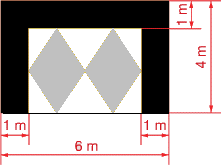
\includegraphics[]{img/lasure.png} 
\end{center}
\end{exercise}

\begin{exercise}
    \textbf{Sur cette feuille.} Dessine dans le réseau de cubes le montage suivant. 
      \begin{center}
          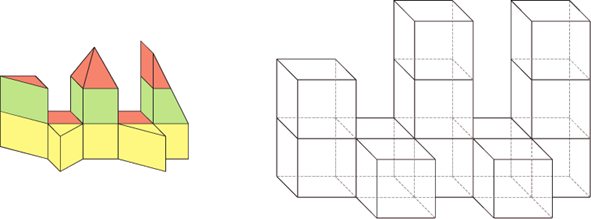
\includegraphics[]{img/cubes.png}
      \end{center}
  \end{exercise}

\end{document}